%!TEX TS-program = xelatex
\documentclass[10pt,oneside]{article}

\usepackage[english]{babel}

\usepackage{amsmath,amssymb,amsfonts}
\usepackage[utf8]{inputenc}
\usepackage[T1]{fontenc}
\usepackage{stix}
\usepackage[scaled]{helvet}
\usepackage[scaled]{inconsolata}

\usepackage{lastpage}

\usepackage{setspace}

\usepackage{ccicons}

\usepackage[hang,flushmargin]{footmisc}

\usepackage{geometry}

\setlength{\parindent}{0pt}
\setlength{\parskip}{6pt plus 2pt minus 1pt}

\usepackage{fancyhdr}
\renewcommand{\headrulewidth}{0pt}\providecommand{\tightlist}{%
  \setlength{\itemsep}{0pt}\setlength{\parskip}{0pt}}

\makeatletter
\newcounter{tableno}
\newenvironment{tablenos:no-prefix-table-caption}{
  \caption@ifcompatibility{}{
    \let\oldthetable\thetable
    \let\oldtheHtable\theHtable
    \renewcommand{\thetable}{tableno:\thetableno}
    \renewcommand{\theHtable}{tableno:\thetableno}
    \stepcounter{tableno}
    \captionsetup{labelformat=empty}
  }
}{
  \caption@ifcompatibility{}{
    \captionsetup{labelformat=default}
    \let\thetable\oldthetable
    \let\theHtable\oldtheHtable
    \addtocounter{table}{-1}
  }
}
\makeatother

\usepackage{array}
\newcommand{\PreserveBackslash}[1]{\let\temp=\\#1\let\\=\temp}
\let\PBS=\PreserveBackslash

\usepackage[breaklinks=true]{hyperref}
\hypersetup{colorlinks,%
citecolor=blue,%
filecolor=blue,%
linkcolor=blue,%
urlcolor=blue}
\usepackage{url}

\usepackage{caption}
\setcounter{secnumdepth}{0}
\usepackage{cleveref}

\usepackage{graphicx}
\makeatletter
\def\maxwidth{\ifdim\Gin@nat@width>\linewidth\linewidth
\else\Gin@nat@width\fi}
\makeatother
\let\Oldincludegraphics\includegraphics
\renewcommand{\includegraphics}[1]{\Oldincludegraphics[width=\maxwidth]{#1}}

\usepackage{longtable}
\usepackage{booktabs}

\usepackage{color}
\usepackage{fancyvrb}
\newcommand{\VerbBar}{|}
\newcommand{\VERB}{\Verb[commandchars=\\\{\}]}
\DefineVerbatimEnvironment{Highlighting}{Verbatim}{commandchars=\\\{\}}
% Add ',fontsize=\small' for more characters per line
\usepackage{framed}
\definecolor{shadecolor}{RGB}{248,248,248}
\newenvironment{Shaded}{\begin{snugshade}}{\end{snugshade}}
\newcommand{\KeywordTok}[1]{\textcolor[rgb]{0.13,0.29,0.53}{\textbf{#1}}}
\newcommand{\DataTypeTok}[1]{\textcolor[rgb]{0.13,0.29,0.53}{#1}}
\newcommand{\DecValTok}[1]{\textcolor[rgb]{0.00,0.00,0.81}{#1}}
\newcommand{\BaseNTok}[1]{\textcolor[rgb]{0.00,0.00,0.81}{#1}}
\newcommand{\FloatTok}[1]{\textcolor[rgb]{0.00,0.00,0.81}{#1}}
\newcommand{\ConstantTok}[1]{\textcolor[rgb]{0.00,0.00,0.00}{#1}}
\newcommand{\CharTok}[1]{\textcolor[rgb]{0.31,0.60,0.02}{#1}}
\newcommand{\SpecialCharTok}[1]{\textcolor[rgb]{0.00,0.00,0.00}{#1}}
\newcommand{\StringTok}[1]{\textcolor[rgb]{0.31,0.60,0.02}{#1}}
\newcommand{\VerbatimStringTok}[1]{\textcolor[rgb]{0.31,0.60,0.02}{#1}}
\newcommand{\SpecialStringTok}[1]{\textcolor[rgb]{0.31,0.60,0.02}{#1}}
\newcommand{\ImportTok}[1]{#1}
\newcommand{\CommentTok}[1]{\textcolor[rgb]{0.56,0.35,0.01}{\textit{#1}}}
\newcommand{\DocumentationTok}[1]{\textcolor[rgb]{0.56,0.35,0.01}{\textbf{\textit{#1}}}}
\newcommand{\AnnotationTok}[1]{\textcolor[rgb]{0.56,0.35,0.01}{\textbf{\textit{#1}}}}
\newcommand{\CommentVarTok}[1]{\textcolor[rgb]{0.56,0.35,0.01}{\textbf{\textit{#1}}}}
\newcommand{\OtherTok}[1]{\textcolor[rgb]{0.56,0.35,0.01}{#1}}
\newcommand{\FunctionTok}[1]{\textcolor[rgb]{0.00,0.00,0.00}{#1}}
\newcommand{\VariableTok}[1]{\textcolor[rgb]{0.00,0.00,0.00}{#1}}
\newcommand{\ControlFlowTok}[1]{\textcolor[rgb]{0.13,0.29,0.53}{\textbf{#1}}}
\newcommand{\OperatorTok}[1]{\textcolor[rgb]{0.81,0.36,0.00}{\textbf{#1}}}
\newcommand{\BuiltInTok}[1]{#1}
\newcommand{\ExtensionTok}[1]{#1}
\newcommand{\PreprocessorTok}[1]{\textcolor[rgb]{0.56,0.35,0.01}{\textit{#1}}}
\newcommand{\AttributeTok}[1]{\textcolor[rgb]{0.77,0.63,0.00}{#1}}
\newcommand{\RegionMarkerTok}[1]{#1}
\newcommand{\InformationTok}[1]{\textcolor[rgb]{0.56,0.35,0.01}{\textbf{\textit{#1}}}}
\newcommand{\WarningTok}[1]{\textcolor[rgb]{0.56,0.35,0.01}{\textbf{\textit{#1}}}}
\newcommand{\AlertTok}[1]{\textcolor[rgb]{0.94,0.16,0.16}{#1}}
\newcommand{\ErrorTok}[1]{\textcolor[rgb]{0.64,0.00,0.00}{\textbf{#1}}}
\newcommand{\NormalTok}[1]{#1}

\newlength{\cslhangindent}
\setlength{\cslhangindent}{1.5em}
\newlength{\csllabelwidth}
\setlength{\csllabelwidth}{3em}
\newenvironment{CSLReferences}[3] % #1 hanging-ident, #2 entry spacing
 {% don't indent paragraphs
  \setlength{\parindent}{0pt}
  % turn on hanging indent if param 1 is 1
  \ifodd #1 \everypar{\setlength{\hangindent}{\cslhangindent}}\ignorespaces\fi
  % set entry spacing
  \ifnum #2 > 0
  \setlength{\parskip}{#2\baselineskip}
  \fi
 }%
 {}
\usepackage{calc} % for \widthof, \maxof
\newcommand{\CSLBlock}[1]{#1\hfill\break}
\newcommand{\CSLLeftMargin}[1]{\parbox[t]{\maxof{\widthof{#1}}{\csllabelwidth}}{#1}}
\newcommand{\CSLRightInline}[1]{\parbox[t]{\linewidth}{#1}}
\newcommand{\CSLIndent}[1]{\hspace{\cslhangindent}#1}\usepackage[table,dvipsnames]{xcolor}

\geometry{includemp,
            letterpaper,
            top=1.2in,
            bottom=2.510cm,
            inner=0.5in,
            outer=0.4in,
            marginparwidth=1.95in,
            marginparsep=0.4in}

\usepackage[singlelinecheck=off]{caption}
\captionsetup{
  font={small},
  labelfont={bf},
  format=plain,
  labelsep=quad
}
\usepackage{floatrow}
\floatsetup[figure]{margins=hangright,
              facing=no,
              capposition=beside,
              capbesideposition={center,outside},
              floatwidth=\textwidth}
\floatsetup[table]{margins=hangoutside,
             facing=yes,
             capposition=beside,
             capbesideposition={center,outside},
             floatwidth=\textwidth}

\pagestyle{plain}

\setcounter{secnumdepth}{5}

\usepackage{titlesec}

\titleformat{\section}[block]
{\normalfont\large\sffamily}
{\thesection}{.5em}{\titlerule\\[.8ex]\bfseries}

\titleformat{\subsection}[runin]
{\normalfont\fontseries{b}\selectfont\filright\sffamily}
{\thesubsection.}{.5em}{}

\titleformat{\subsubsection}[runin]
{\normalfont\itshape\rmfamily\bfseries}{\thesubsubsection}{1em}{}

\fancypagestyle{firstpage}
{
   \fancyhf{}
   \renewcommand{\headrulewidth}{0pt}
   \fancyfoot[R]{\footnotesize\ccby}
   \fancyfoot[L]{\footnotesize\sffamily\today}
}

\fancypagestyle{normal}
{
  \fancyhf{}
  \fancyfoot[R]{\footnotesize\sffamily\thepage\ of \pageref*{LastPage}}
}

\usepackage{tikz}
\begin{document}
\pagestyle{normal}
\thispagestyle{firstpage}

\newcommand{\colorRule}[3][black]{\textcolor[HTML]{#1}{\rule{#2}{#3}}}

\noindent {\LARGE \textbf{\textsf{Using simulation models to infer
ecological mechanisms}}}

\medskip
\begin{flushleft}
{\small
%
\href{https://orcid.org/0000-0002-6506-6487}{M.D.\,Catchen}%
%
\,\textsuperscript{1,2}
\vskip 1em
\textsuperscript{1}\,McGill University; \textsuperscript{2}\,Québec
Centre for Biodiversity Sciences\\
\vskip 1em
\textbf{Correspondance to:}\\
}
\end{flushleft}

\vskip 2em
\makebox[0pt][l]{\colorRule[CCCCCC]{2.0\textwidth}{0.5pt}}
\vskip 2em
\noindent

\marginpar{\vskip 1em\flushright
{\small{\bfseries Keywords}:\par
computational ecology\\simulation\\likelihood-free
inference\\approximate bayesian computation\\}
}


\textbf{Abstract}:\,ch1 of my dissertation in paper form

\vskip 2em
\makebox[0pt][l]{\colorRule[CCCCCC]{2.0\textwidth}{0.5pt}}
\vskip 2em

\hypertarget{introduction}{%
\section{Introduction}\label{introduction}}

Earth's ecosystems are immensely variable---they are the emergent result
of biological processes that exist across spatial, temporal, and
organizational scales (Levin 1992). These processes enable, influence
and compound on one another, resulting in the immense diversity of
functions and forms of life on Earth. There has been a longstanding
debate if there is any \emph{generality}, or better \emph{universality},
to these processes (\textbf{Lawton1999?}). Answering this question, even
in abstract, proves difficult. How can we determine if there is some set
of universal rules or mechanisms that underlie systems driven by many
factors which interact in nonlinear and probabilistic ways across
separate organizational scales? We propose that this problem can be
split into two parts: 1) deciding on the best spatial, temporal, and
organizational scale at which to model an ecosystem process, and 2)
after a particular scale has been chosen, determining the best model at
that scale and associated parameters that explain a particular dataset.

The first question is to determine the proper scale to model a given
system. Innumerable biological mechanisms have been posited at various
spatial, temporal, and organizational scales (fig.~\ref{fig:slices}).
How does one decide the best scale at which to model a processes, or at
what scale it is best to look for universality?

(\textbf{LevinsLewontin?}) write

\begin{quote}
The problem for science is to understand the proper domain of
explanation of each abstraction rather than become its prisoner.
\end{quote}

The second question is, after a given scale is selected, to select the
best model from a set of competing models at that scale. This question
is primarily implicated with prediction---that is, what model best
predicts ecological systems at a particular scale? This has applied need
as forecasting is an imperative in ecology. Some scales are more
predictable than others.

\begin{figure}
\hypertarget{fig:slices}{%
\centering
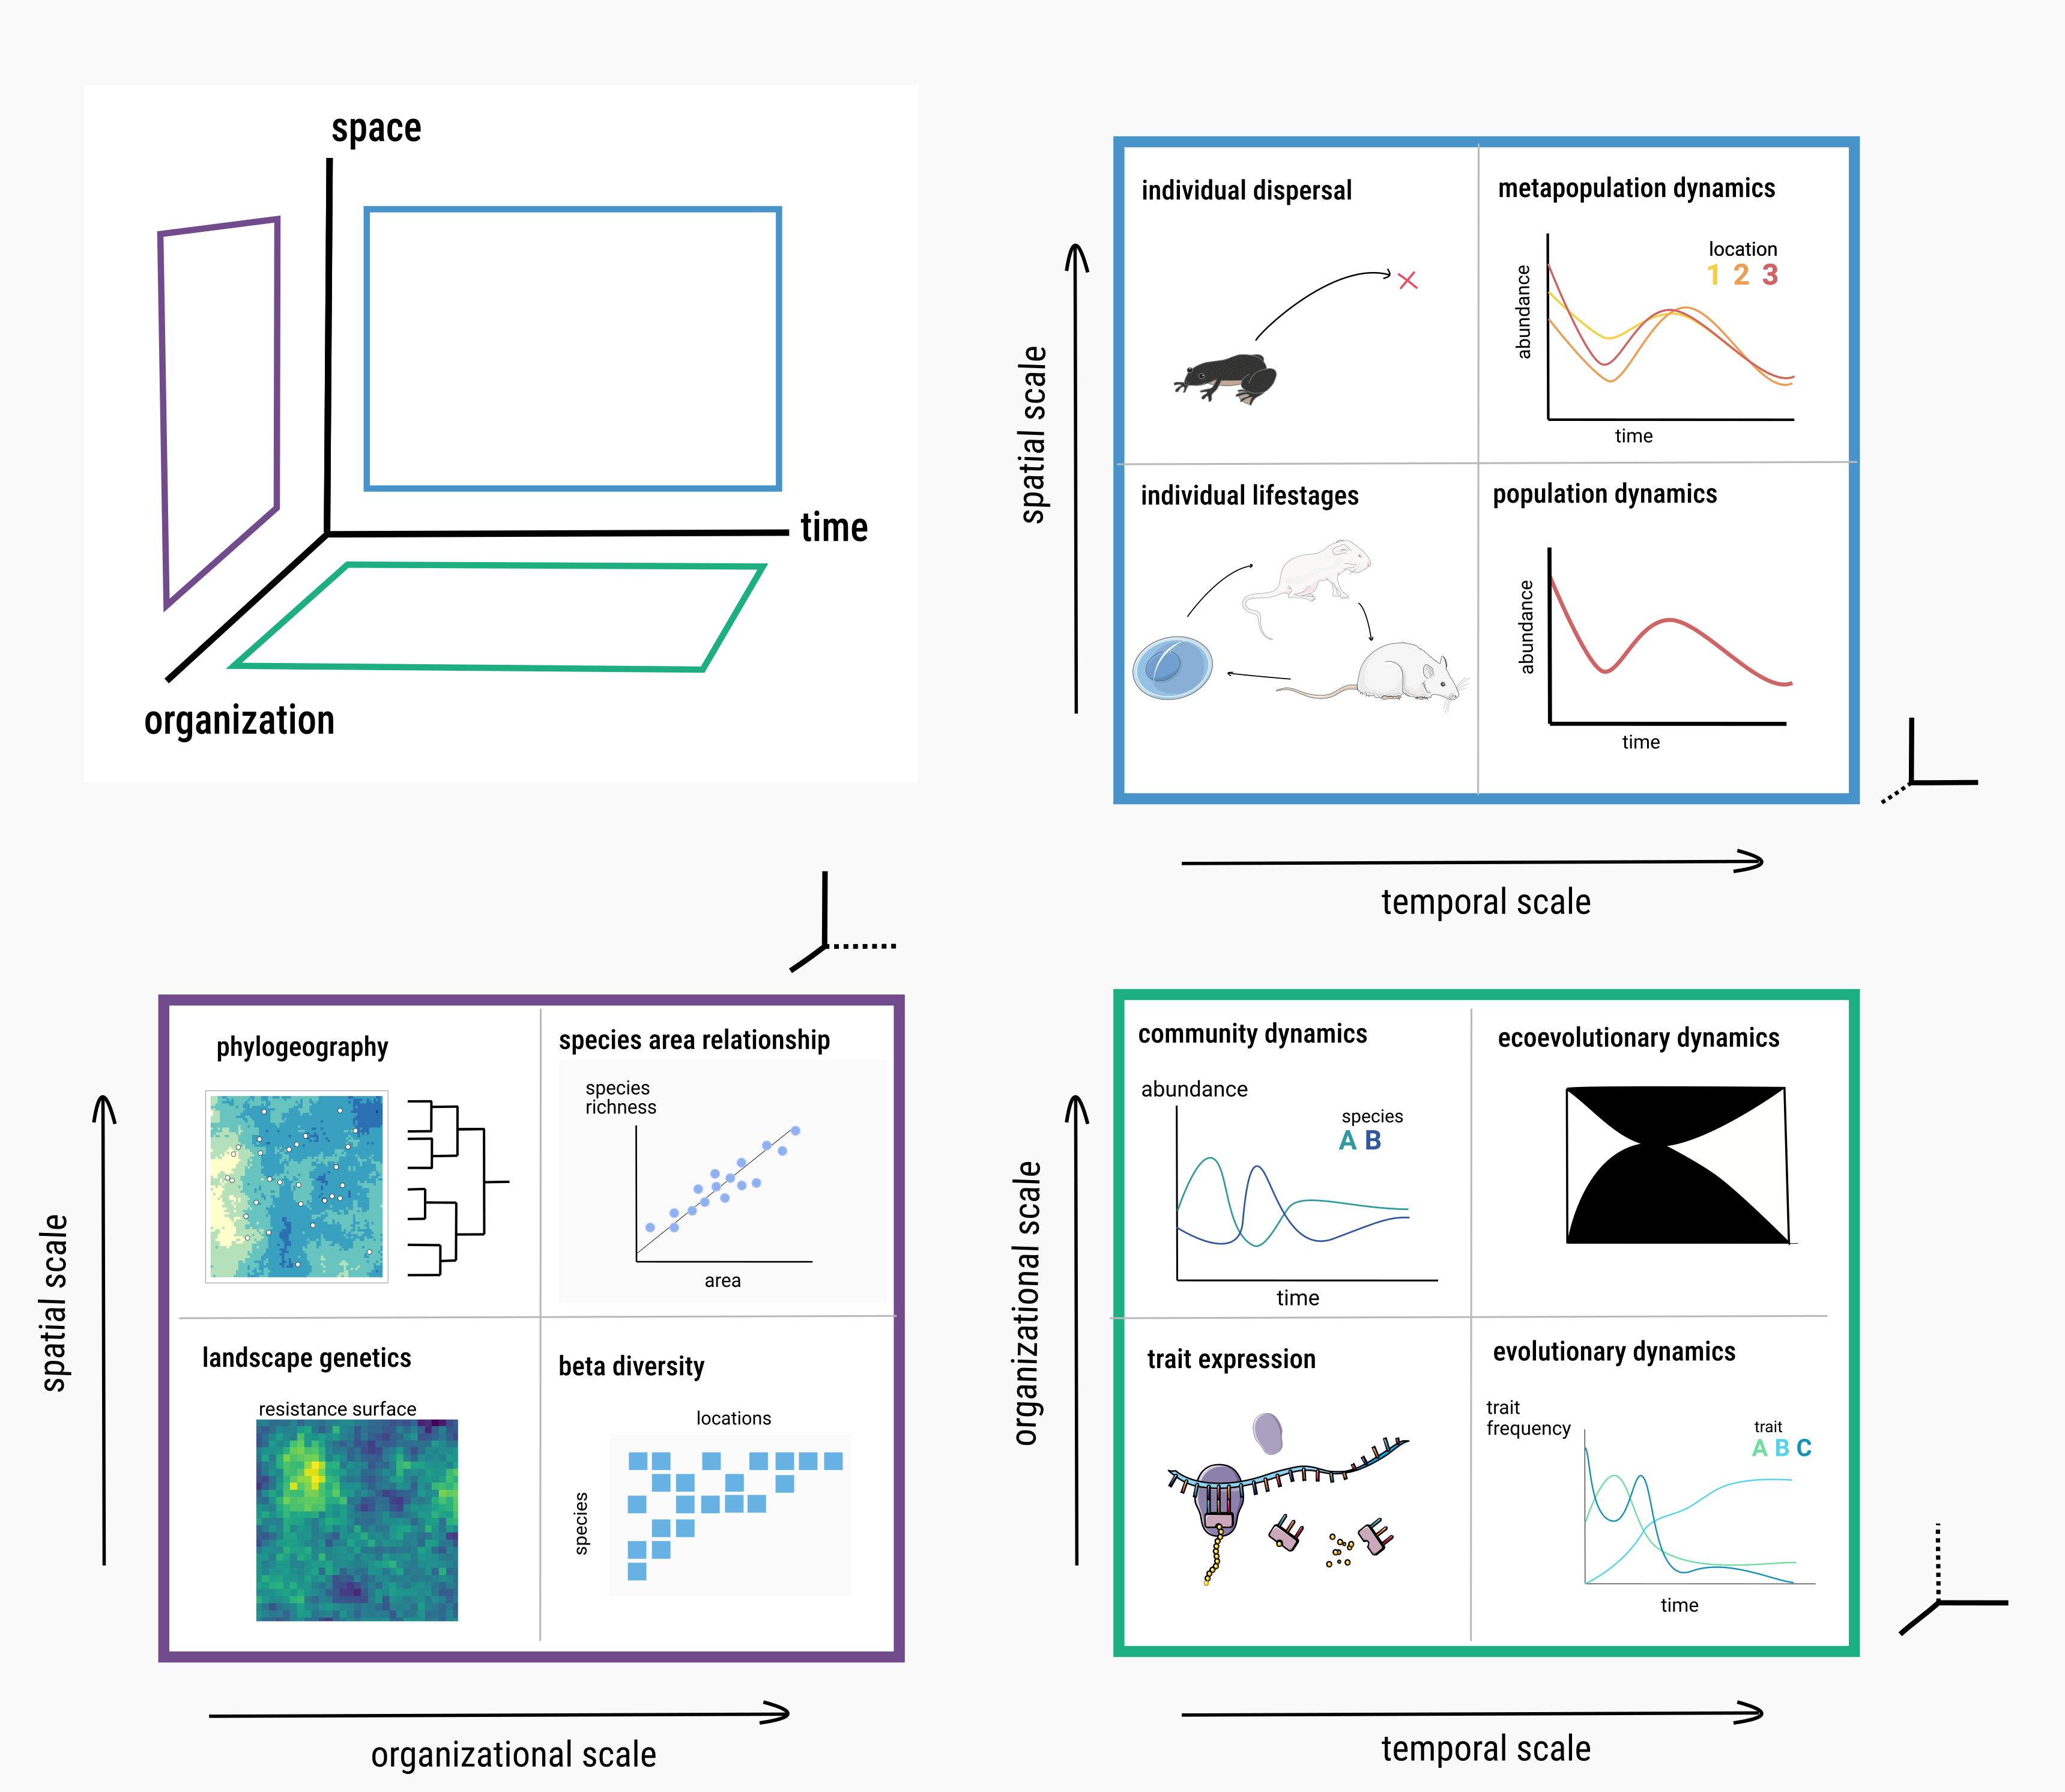
\includegraphics{./figures/tensorslices.png}
\caption{Conceptual space with three axes.}\label{fig:slices}
}
\end{figure}

(\textbf{Lawton1999?}) argues that as an organizational scale, the
ecology community is frought with too many ``contingencies'' in order to
find universality. Partially in response to Lawton's paper, the
metacommunity framework (\textbf{Leibold2003MetCom?}) sought to address
the inherently spatial nature of metacommunity processes. Vellend (2010)
posits four fundamental processes, analogous to evolutionary genetics.
(\textbf{Poisot2015BeySpe?}) also notes the importance of variation in
traits and abundance. Necessary additional spatial and temporal
dimension to community processes. The scales at which we propose
mechanisms are subject to selection bias based on the data we can
collect---looking for lost keys where the light is better.

The data we collect from ecological systems is inherently noisy. This
data contains information produced by a combination of the amalgamation
of ``true'' ecological and evolutionary mechanisms (interacting in
unknown ways) compounded by sampling biases.

What is in this paper? We argue that advances in computational resources
and methods for likelihood-free inference put us in the place where
simulation models can enable us to test more complex interaction
mechanisms (Cranmer, Brehmer, and Louppe 2020). We present a conceptual
framework for determining the best model from a set of competing
simulation models. We then present an example where we fit data from
LTER wisconsin fish to both individual-species level and community level
simulation models to determine which provides better predictions about
occupancy over time. ScientificML (Rackauckas et al. 2020).

\hypertarget{a-state-space-perspective-on-ecological-mechanisms}{%
\section{A state-space perspective on ecological
mechanisms}\label{a-state-space-perspective-on-ecological-mechanisms}}

In order to present the conceptual framework for simulation-based
inference, we first need to propose some definitions. This conceptual
framework is based around consider the \emph{dynamics} of a
metacommunity system by considering the \emph{geometry} of how that
system changes in \emph{state-space}.

Dynamical systems is the subfield of mathematics related to systems that
change over time. Often by applying a geometric perspective to
state-space. What is state space?

\textbf{\emph{What is an ecological mechanism?}} A mechanism describes
how the state of a system changes from one timestep to the next.\\
A mapping between low dimensional latent/parameter space and information
space.

Why is simulation necessary in ecology? They allow us to produce data
that encodes explicit mechanism (Crutchfield 1992).

\textbf{\emph{Metacommunity states and mechanisms}} Within this
abstraction, a metacommunity state is a set of measurements for species
across locations at a single point in time, which can be represented as
a matrix: a grid of measurements where each row corresponds to location
and each column to species.

\textbf{\emph{Metacommunity dynamics and tensors}} Across timepoints, a
set of states form trajectories which can be represented as a a tensor.

\begin{figure}
\hypertarget{fig:flow}{%
\centering
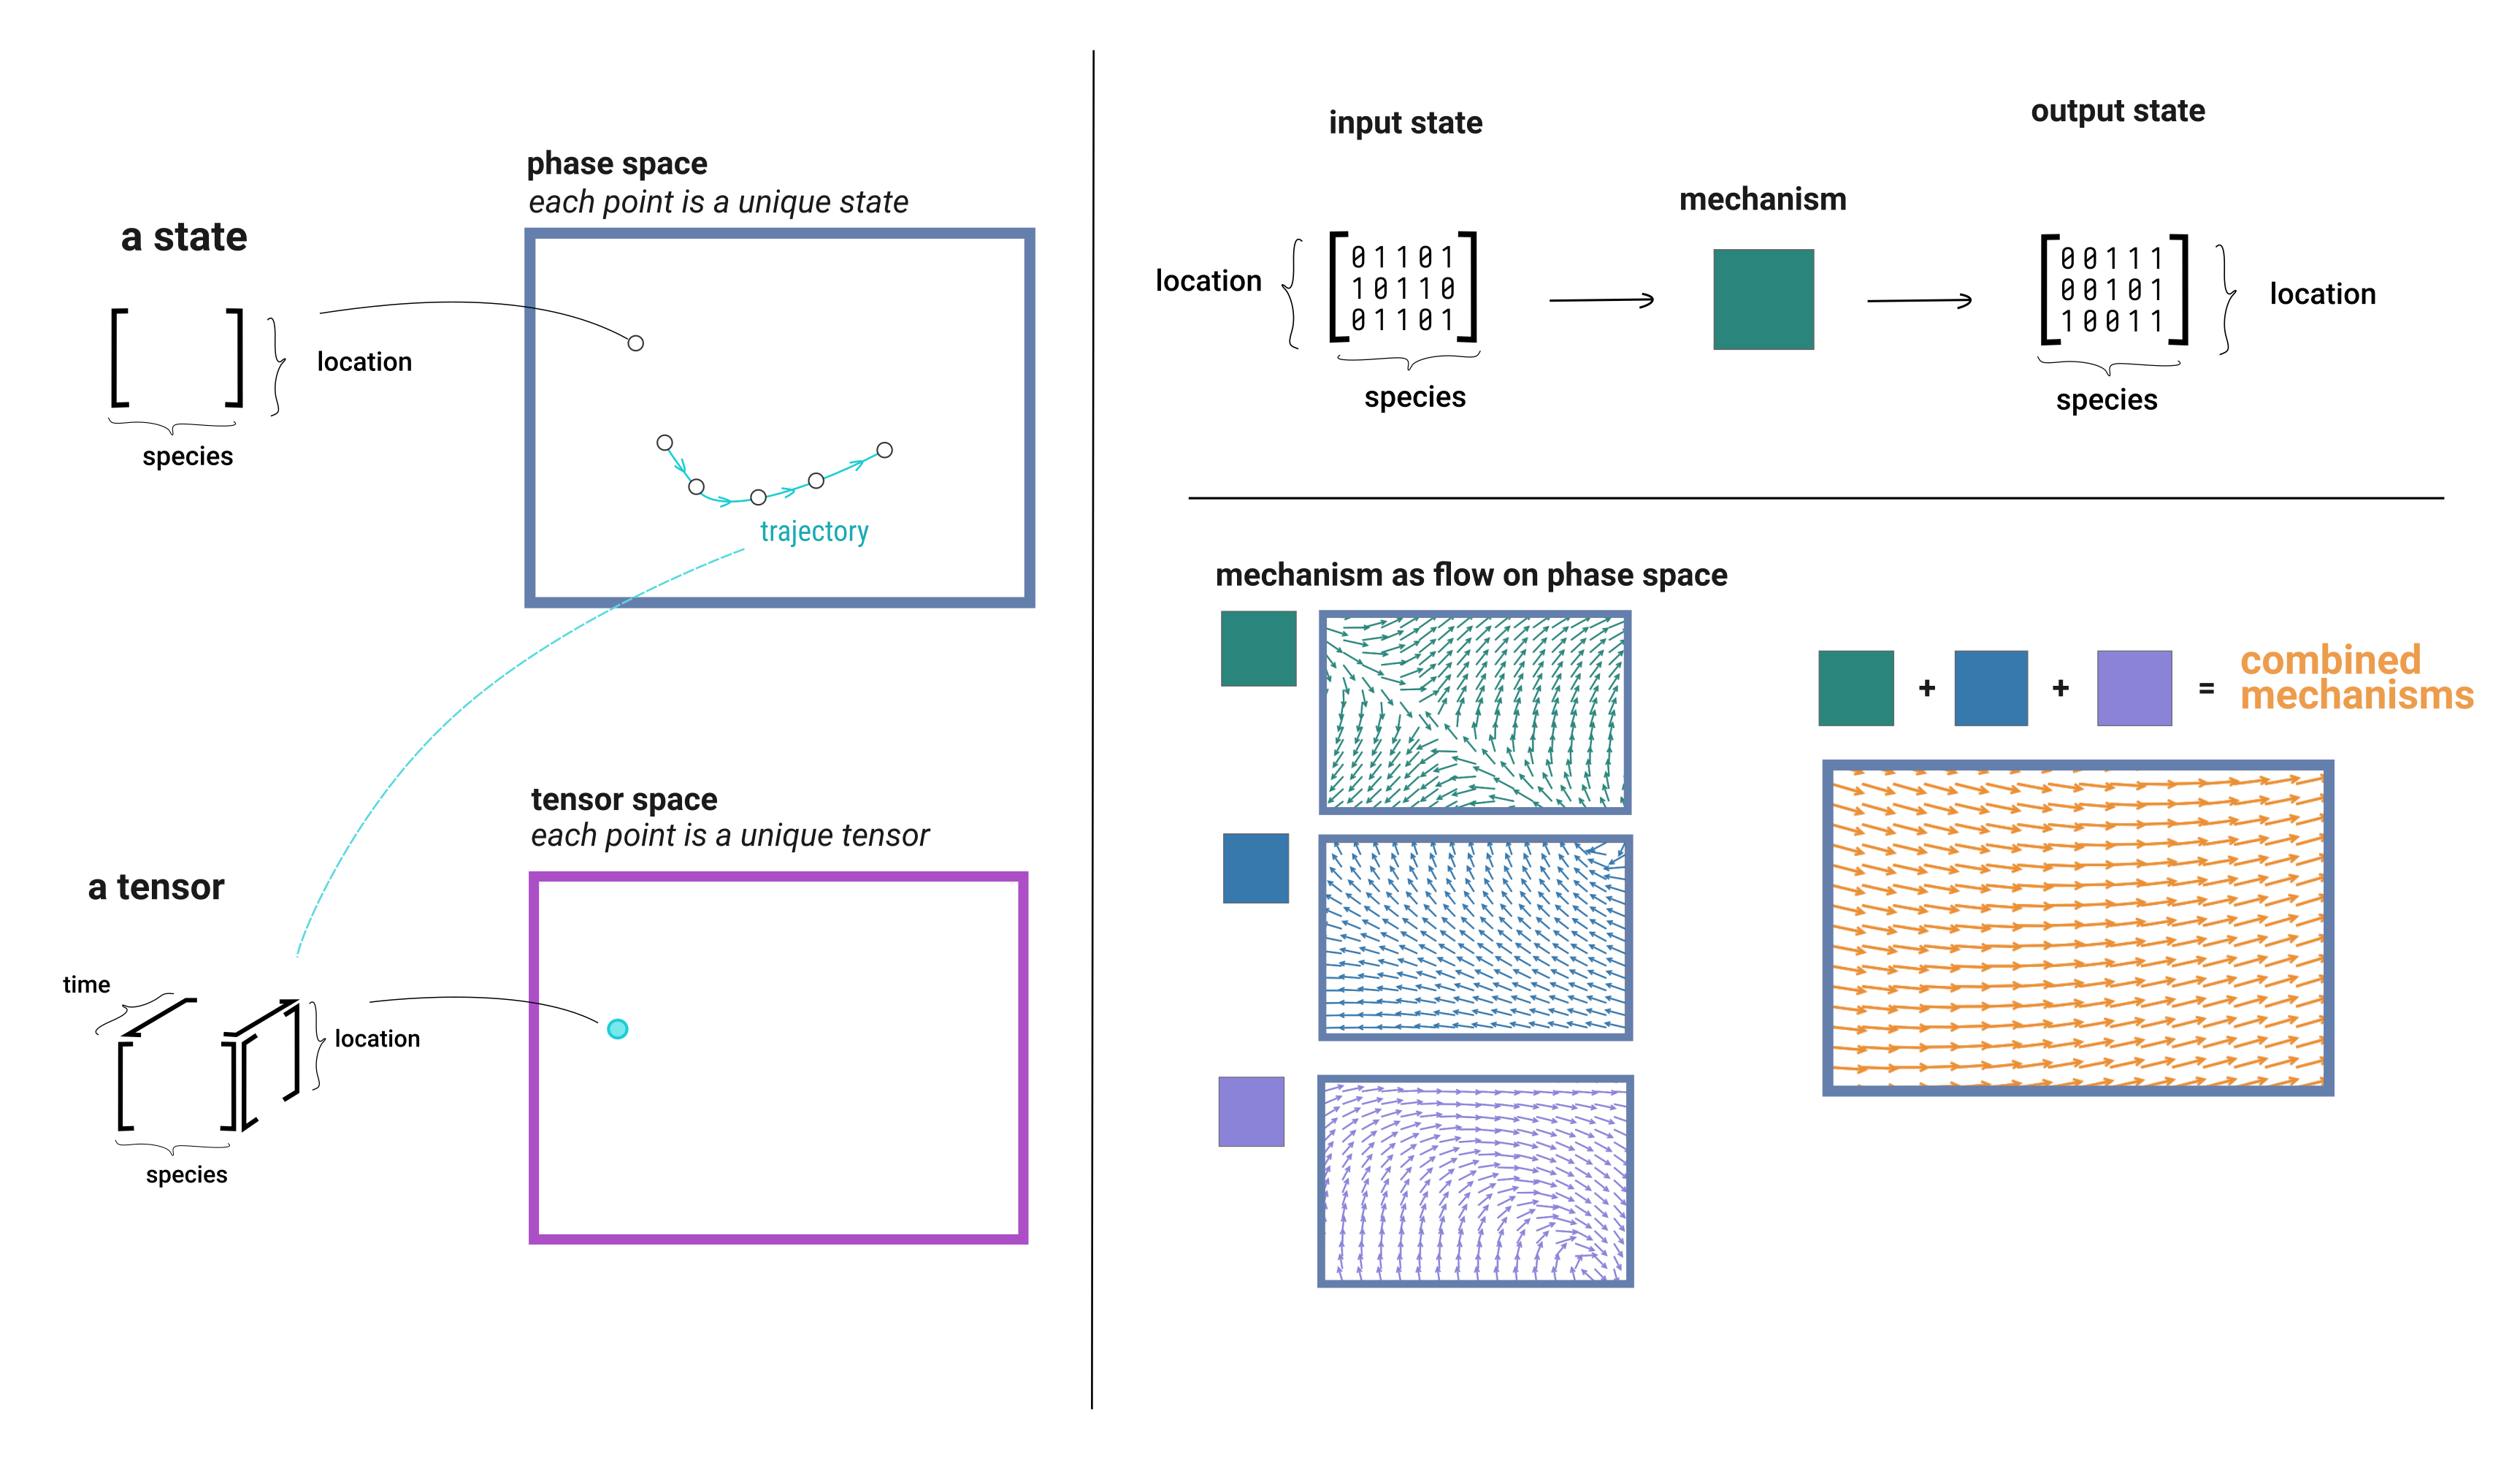
\includegraphics{./figures/flows.png}
\caption{A mechanism is a flow on the state space.}\label{fig:flow}
}
\end{figure}

\hypertarget{using-simulation-to-infer-mechanisms-in-ecology}{%
\section{Using simulation to infer mechanisms in
ecology}\label{using-simulation-to-infer-mechanisms-in-ecology}}

Simulation models have a long history in ecology. cite some examples.

Still, fitting simulation models to data is difficult. \^{}what does
this mean to someone who doesn't know what fitting means

No likelihood function. General problem of high-dimensional model,
compounded by little data.

What is enabling this now? computational capacity and methods for
optimization parameter estimation. More data.

\begin{figure}
\hypertarget{fig:information}{%
\centering
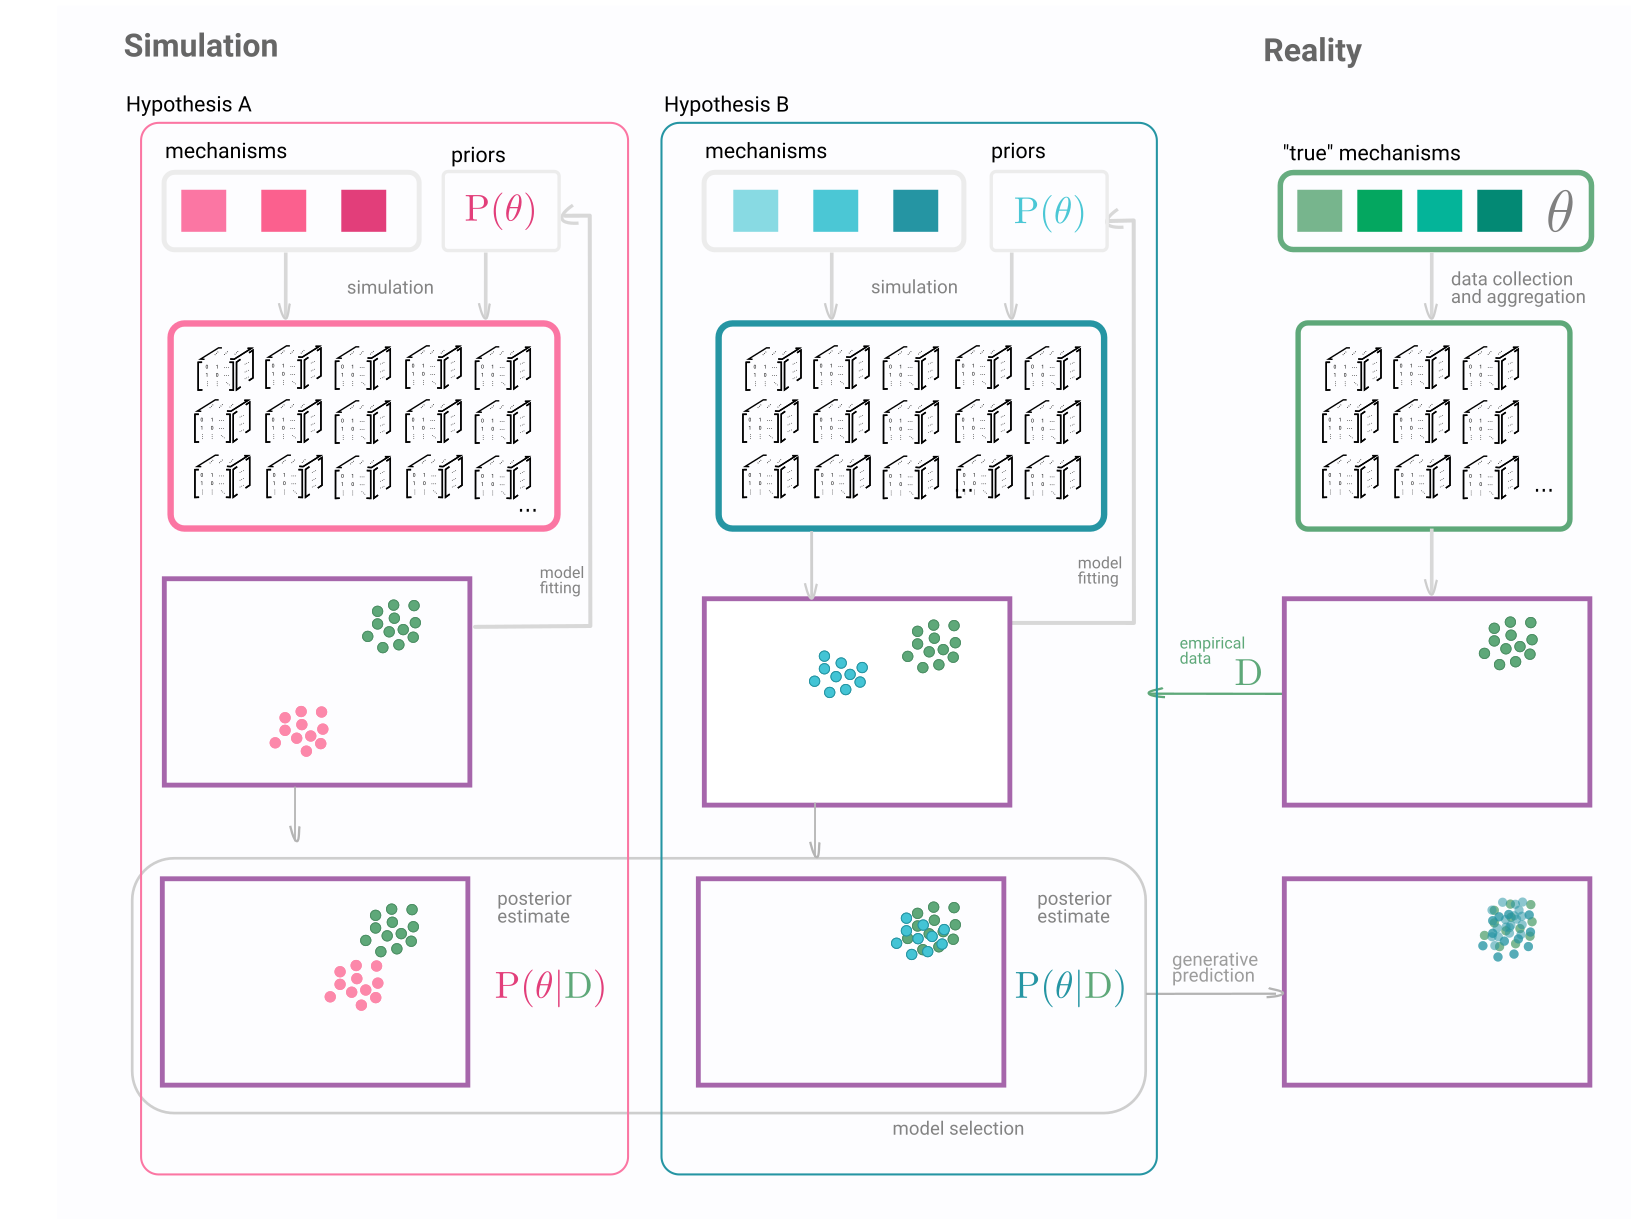
\includegraphics{./figures/likelihoodfreeinference.png}
\caption{Likelihood free inference for metacommunity
ecology}\label{fig:information}
}
\end{figure}

\hypertarget{case-study-species-versus-community-level-occupancy-models}{%
\section{Case study: species versus community level occupancy
models}\label{case-study-species-versus-community-level-occupancy-models}}

In this section we use data from LTER Minnesota lakes for five fish
species. We look at the occupancy dynamics of five species (list
species) across NS sites for each year from 198something-200something.
We fit two simulation models via likelihood-free inference: first where
each species exhibit independent occupancy dynamics, and second where
each species has the same \(c\) and \(e\) value.

\textbf{\emph{Independent Species Model}} We simulate dynamics where
each species \(i\) has a colonization probability \(c_i\) and an
extinction probability \(e_i\). These are assumed to be a fixed value
for each species which does not vary over time.

\textbf{\emph{Unified Model}} The colonization for each species \(i\) is
\(c\), extinction probability is \(e\).

\begin{figure}
\hypertarget{fig:abcfit}{%
\centering
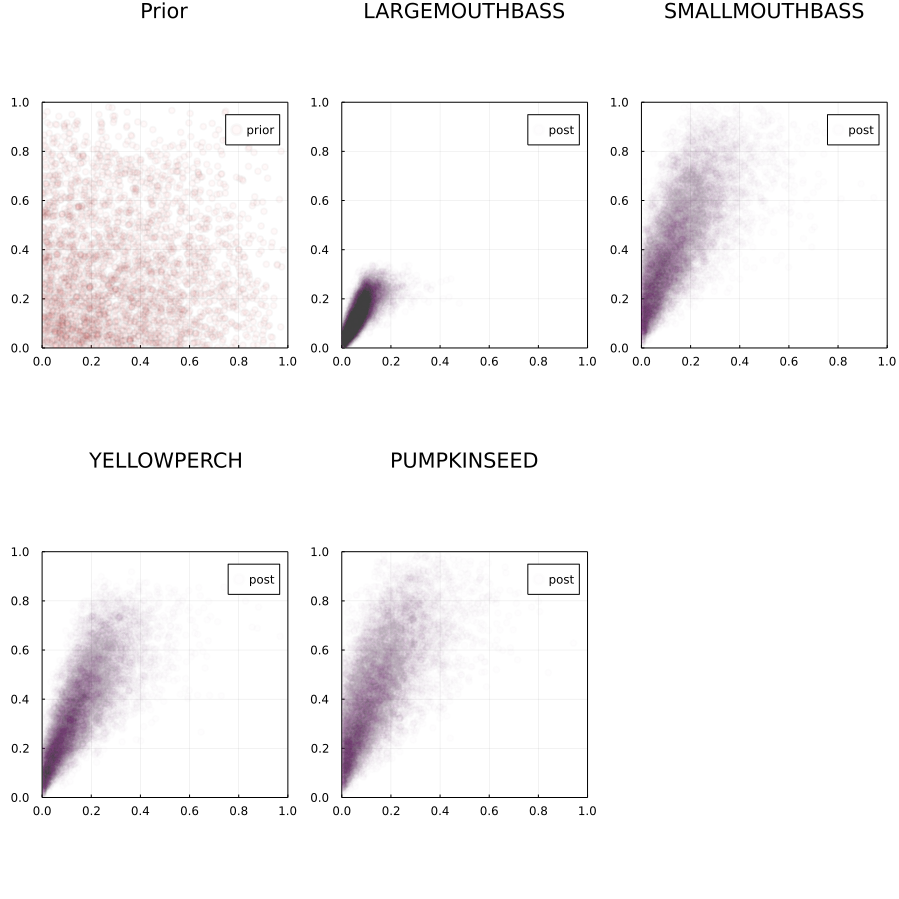
\includegraphics{./figures/abcfit.png}
\caption{here's the fit as of now for individual
species}\label{fig:abcfit}
}
\end{figure}

\textbf{\emph{Results figure}} Panel A: AUC-ROC for single species
prediction Panel B: AUC-ROC for unified prediction Panel C: Mean error
for proportion occupancy for each model.

\textbf{\emph{Assessing fit}}

Test it on simulated data to see if it works.
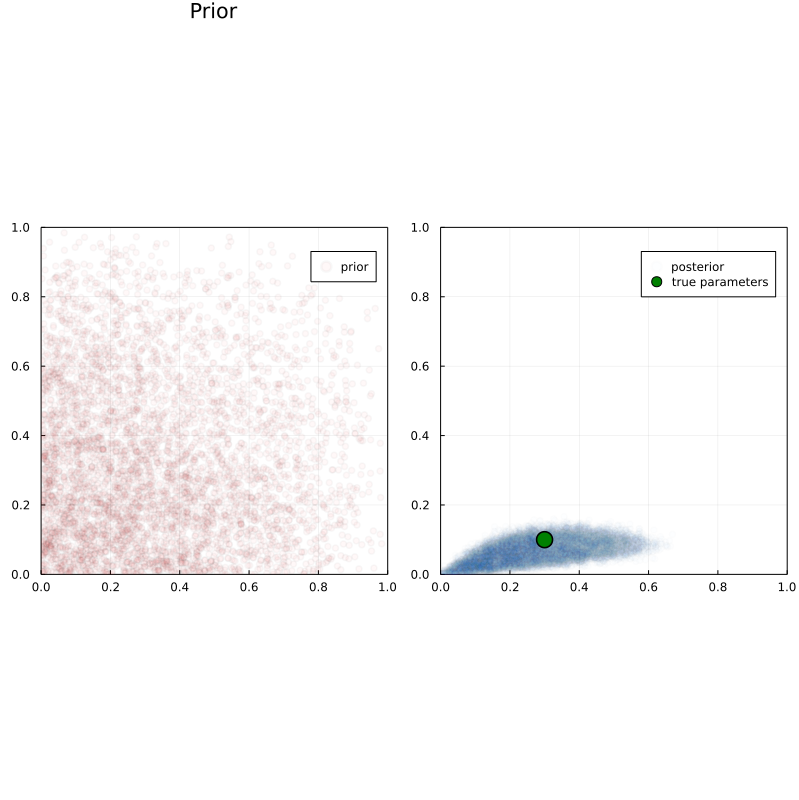
\includegraphics{./figures/comparedtotruth.png}

\textbf{\emph{We need to talk about summary statistics}}

Is proportion more ``predictable'' than individual occupancy?

Which ones make effective predictions? What models do we use to fit
empirical data to simulated (generative adversarial networks, MCMC-ABC
methods, etc.)

Caveats on more complex models for this simple example. Refer to
up-to-date resources on model fitting an assessment.

\hypertarget{predictive-ecology-as-a-scientific-epistemology}{%
\section{Predictive ecology as a scientific
epistemology}\label{predictive-ecology-as-a-scientific-epistemology}}

What scales are inherently more predictable.

Here we propose that simulation models have the potential to infer This
results in the question: what are the mechanisms best describe a set of
data?

Science is fundamentally a theory of epistemology: a methodology and set
of principles to make justified claims about the world. Descriptive
claims about the world (the Earth goes around the sun, more species are
found near the equator than far from it) are considered justified if
they make predictions that agree with observed reality.

\begin{quote}
The sciences do not try to explain, they hardly even try to interpret,
they mainly make models. By a model is meant a mathematical construct
which, with the addition of certain verbal interpretations, describes
observed phenomena. The justification of such a mathematical construct
is solely and precisely that it is expected to work - that is correctly
to describe phenomena from a reasonably wide area. Furthermore, it must
satisfy certain esthetic criteria - that is, in relation to how much it
describes, it must be rather simple.

John Von Neumann
\end{quote}

\begin{quote}
The electron is a theory we use; it is so useful in understanding the
way nature works that we can almost call it real.

Richard P. Feynman
\end{quote}

The whole idea of searching for ``laws'' (Lawton) rests on an assumption
that there are universal

All models are wrong is not just about statistical models.

In order to determine if a descriptive claim agrees with reality, it
must be translated into a quantitative model that makes predictions
about things that can be measured. These quantitative models take many
forms. A subclass of these models, mechanistic models, represent latent
processes that can not be observed or measured, either inherently or due
to technological limitations.

Different levels of conceptual abstraction have proven successful in
predicting how biological systems change over time.

Still, predicting how ecosystems will change in the future remains a
fundamental goal of ecology.

There is variation in the what scales are best for prediction (Brodie et
al. 2021), and some forms of dynamics are intrinsically complex enough
to avoid effective prediction at all (Pennekamp et al. 2019; Beckage,
Gross, and Kauffman 2011; Chen, Angulo, and Liu 2019).

\hypertarget{conclusion}{%
\section{Conclusion}\label{conclusion}}

What does is mean for a model to be correct? Take the logistic model,
for example. Although logistic growth is observed in many model and to
some degree non-model systems, it is hard to say there is some intrinsic
truth to this--i.e. that logistic growth is an ecoloigical ``law.'' The
phenomena of population dynamics are the result of individual organisms
being born, reproducing, and dying at a lower level of organization, but
the logistic model is a useful abstraction under some circumstances.

It is useful the notion that a model represents some ``truth'' about the
world, instead models have vary in their usefulness. predictive accuracy
is one measure of this usefulness. The problem is you cannot tell the
difference ---Hume and the induction problem.

If a simulation makes data the looks like real data, does it represent
the ``true'' world? Does it matter? Newtonian Gravity was ``right,''
until GR was more right. Different models at different levels of
abstract provide varying levels of predictive accuracy. Mechanisms that
are incorrect that produce information that shares statistical
properties with empirical data can still be useful.

\textbf{\emph{What are the limitations of the utility of mechanistic
simulations}} There are limits to the scope of simulation models. How do
we know when they are appropriate, versus a ML/non-mechanistic model?
Need for flexible set of tools to do this, setting up the next chapter.

\hypertarget{references}{%
\section*{References}\label{references}}
\addcontentsline{toc}{section}{References}

\hypertarget{refs}{}
\begin{CSLReferences}{1}{0}
\leavevmode\hypertarget{ref-Beckage2011LimPre}{}%
Beckage, Brian, Louis J. Gross, and Stuart Kauffman. 2011. {``The Limits
to Prediction in Ecological Systems.''} \emph{Ecosphere} 2 (11): art125.
\url{https://doi.org/10.1890/ES11-00211.1}.

\leavevmode\hypertarget{ref-Brodie2021ExpTim}{}%
Brodie, Stephanie, Briana Abrahms, Steven J. Bograd, Gemma Carroll,
Elliott L. Hazen, Barbara A. Muhling, Mercedes Pozo Buil, James A.
Smith, Heather Welch, and Michael G. Jacox. 2021. {``Exploring
Timescales of Predictability in Species Distributions.''}
\emph{Ecography} 44 (6): 832--44.
\url{https://doi.org/10.1111/ecog.05504}.

\leavevmode\hypertarget{ref-Chen2019RevCom}{}%
Chen, Yize, Marco Tulio Angulo, and Yang-Yu Liu. 2019. {``Revealing
Complex Ecological Dynamics via Symbolic Regression.''} \emph{BioEssays}
41 (12): 1900069. \url{https://doi.org/10.1002/bies.201900069}.

\leavevmode\hypertarget{ref-Cranmer2020FroSim}{}%
Cranmer, Kyle, Johann Brehmer, and Gilles Louppe. 2020. {``The Frontier
of Simulation-Based Inference.''} \emph{Proceedings of the National
Academy of Sciences} 117 (48): 30055--62.

\leavevmode\hypertarget{ref-Crutchfield1992SemThe}{}%
Crutchfield, James P. 1992. {``Semantics and Thermodynamics,''} 38.

\leavevmode\hypertarget{ref-Levin1992ProPat}{}%
Levin, Simon A. 1992. {``The Problem of Pattern and Scale in Ecology:
The Robert H. MacArthur Award Lecture.''} \emph{Ecology} 73 (6):
1943--67. \url{https://doi.org/10.2307/1941447}.

\leavevmode\hypertarget{ref-Pennekamp2019IntPre}{}%
Pennekamp, Frank, Alison C. Iles, Joshua Garland, Georgina Brennan,
Ulrich Brose, Ursula Gaedke, Ute Jacob, et al. 2019. {``The Intrinsic
Predictability of Ecological Time Series and Its Potential to Guide
Forecasting.''} \emph{Ecological Monographs} 89 (2): e01359.
\url{https://doi.org/10.1002/ecm.1359}.

\leavevmode\hypertarget{ref-Rackauckas2020UniDif}{}%
Rackauckas, Christopher, Yingbo Ma, Julius Martensen, Collin Warner,
Kirill Zubov, Rohit Supekar, Dominic Skinner, Ali Ramadhan, and Alan
Edelman. 2020. {``Universal Differential Equations for Scientific
Machine Learning.''} \emph{arXiv:2001.04385 {[}cs, Math, q-Bio,
Stat{]}}, August. \url{http://arxiv.org/abs/2001.04385}.

\leavevmode\hypertarget{ref-Vellend2010ConSyn}{}%
Vellend, Mark. 2010. {``Conceptual Synthesis in Community Ecology.''}
\emph{The Quarterly Review of Biology} 85 (2): 183--206.
\url{https://doi.org/10.1086/652373}.

\end{CSLReferences}

\end{document}
